\documentclass[a4paper,11pt, twoside]{article}
\usepackage[english]{babel}
%\usepackage[utf8]{inputenc}
\usepackage{amsmath}
\usepackage{graphicx}
\usepackage{float}
\usepackage{fixltx2e}
\usepackage{listings}
\usepackage{dirtree}
\usepackage{enumitem}
\usepackage{color}
\usepackage{textcomp}
\usepackage{latexsym}
\usepackage{lstautogobble}
\usepackage[colorinlistoftodos]{todonotes}
\usepackage[margin=3cm]{geometry}
\usepackage{hyperref}
\usepackage{fancyhdr}
\usepackage{tikz}
\usetikzlibrary{patterns}
\usetikzlibrary{shapes,positioning,calc}
\usetikzlibrary{shapes.geometric, arrows}
\usetikzlibrary{arrows.meta}
\colorlet{lightgray}{gray!20}
\usepackage{libertine}
\usepackage{csquotes}
\usepackage[backend=bibtex, style=numeric]{biblatex}
\addbibresource{biblio.bib}
\hypersetup{
	hidelinks, 
	colorlinks = true,
	linkcolor = black,
	citecolor = black,
	urlcolor = blue
}
\lstset{
language=Java,
keywordstyle=\color{blue},
showtabs=false,
showspaces=false,
showstringspaces=false,
frame=single,
basicstyle=\ttfamily\small,
breaklines=true
}

\pagestyle{fancy}
\lhead{\nouppercase{\leftmark}}
\rhead{\nouppercase{\rightmark}}
\chead{}
\lfoot{}
\cfoot{\thepage}
\rfoot{}
\renewcommand{\headrulewidth}{0.4pt}
\renewcommand*\DTstylecomment{\rmfamily}

\renewcommand{\ttdefault}{cmtt}
\begin{document}
	\clearpage
	\begin{titlepage}
		\centering
		\vspace*{\fill}
		{\scshape\LARGE Università degli Studi di Verona \par}
		\vspace{1.5cm}
		\line(1,0){240} \\
		{\huge\bfseries Authorship Attribution\par}
		\line(1,0){240} \\
		\vspace{0.5cm}
		{\scshape\Large Big Data project report\par}
		\vspace{2cm}
		{\Large\itshape Davide Bianchi VR424505\par
		\Large\itshape Matteo Danzi VR424987\par}
		\vspace{1cm}
		\vspace{5cm}
		\vspace*{\fill}
		% Bottom of the page
		{\large A.A. 2018/2019\par}
	\end{titlepage}
	\thispagestyle{empty}
	\newpage
	\tableofcontents
	\newpage
	
	\section{Introduction}
	The project aim was to design a tool which could establish the authorship of a manuscript by using specific criteria described later. 
	The used architecture is based on Hadoop, a distributed filesystem simulator, running in a Docker container. The requirements of the project imposed the use of MapReduce programming model as seen in Laboratory Lessons of the Big Data course.

	\section{Background and System Description}
    \subsection{Cloudera Docker and system setup}
		A container is a standard unit of software that packages up code and all its dependencies so the application runs quickly and reliably from one computing environment to another. A Docker container image is an executable package of software that includes everything needed to run an application: code, runtime, system tools, system libraries and settings.

		\bigskip

		\noindent
		Docker images become containers when they run on Docker Engine. They isolate software from its environment and ensure that it works uniformly despite differences for instance between development and staging.
		
		\bigskip

		\noindent
		The Cloudera\parencite{Cloudera} Docker image used in this project contains an Hadoop Distributed File System (HDFS) partition. Cloudera provides a scalable, flexible, integrated platform that makes it easy to manage rapidly increasing volumes and varieties of data in an enterprise. 

		\bigskip
		
		\noindent
		Cloudera provides an HDFS (\textit{Hadoop Distributed FileSystem})\parencite{Hadoop-Mapreduce}, used to store files across server collections. The Hadoop version used in this project is \texttt{Hadoop 2.6.0-cdh5.7.0}.
		
		The distributed filesystem consists on two basic services: \begin{itemize}
			\item \textit{NameNode}: is a single instance service, running on a master node, which is responsible for files and directory mantainance within the filesystem itself;
			
			\item \textit{DataNode}: running on multiple nodes (many instances are allowed), are supposed to retrieve the application data when they are told by the NameNode.
		\end{itemize}
	
		\bigskip
		
		\noindent
		For the installation of Docker, the Cloudera Docker image and the execution of jobs using jar file it have been used the instructions of the course. The project is written using Java version \texttt{11.0.4}. For the code compilation we used IntelliJ version \texttt{2019.2.4} compiling using compatibility mode with version \texttt{1.7}.

	\subsection{Map Reduce Framework}
		MapReduce is a programming paradigm which works on parallel platforms in order to process in the best possible way large amounts of data. The client has to implement a map function, which is supposed to take as input raw data and process them into intermediate \textit{key-value} pairs, and the reduce function, which aim is to regroup key-value pairs relying on the key and generate key-value output pairs. The mapreduce model is explained more in detail in the next section.
		
		\bigskip


		\noindent
		This Programming Model consists of two main actions:
		\begin{itemize}
			\item \textbf{Map}: application of a function to every object in a list. Each object (e.g.: document) is independent.
			\begin{itemize}
				\item Order is not important
				\item Maps can be done in parallel since every object has no relation to each other
				\item The function produces an intermediate result
			\end{itemize}
			
			Formally the \textit{map} function can be described with the following notation: \[ map:(key_1, value_1) \to list(key_2, value_2) \]
			\item \textbf{Reduce}: grouping key-value pairs on key, and combining the intermediate results generated by Maps to produce a final result. Formally the reduce function is defined as \[ reduce:(key_2, list(value_2)) \to (key_3, value_3)  \]
		\end{itemize}

		\begin{figure}[h!]
			\centering
			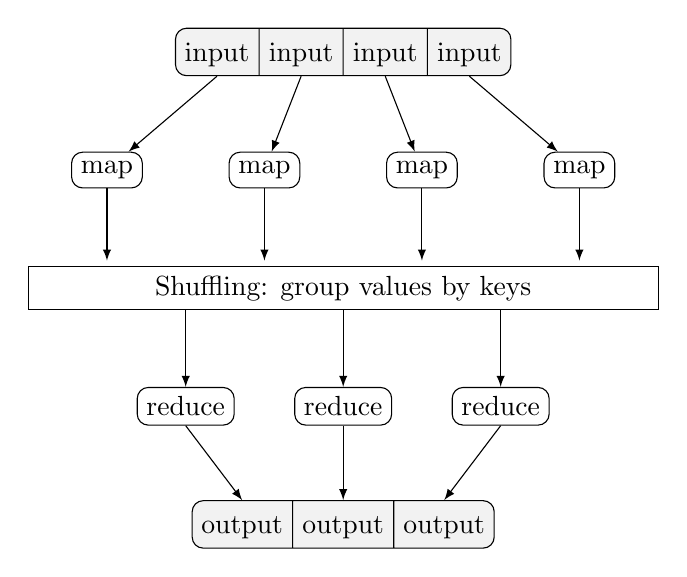
\begin{tikzpicture}[>=latex, relation/.style={rectangle split, rectangle split parts=#1, rectangle split part align=base, draw, anchor=center, align=center, text height=3mm, text centered}]
				% Nodes

				\node [relation=4, rounded corners, rectangle split horizontal, rectangle split part fill={lightgray!50}] (n0) at (0,0)
				{%
					\nodepart{one} input
					\nodepart{two} input
					\nodepart{three} input
					\nodepart{four} input};
				\node [draw, rectangle, rounded corners] (m1) at (-3,-1.5) {map};
				\node [draw, rectangle, rounded corners] (m2) at (-1,-1.5) {map};
				\node [draw, rectangle, rounded corners] (m3) at (1,-1.5) {map};
				\node [draw, rectangle, rounded corners] (m4) at (3,-1.5) {map};
				\draw node[draw, rectangle, minimum width=8cm] (inter) at ($ (n0) +(0,-3) $) {Shuffling: group values by keys};
				\node [draw, rectangle, rounded corners] (r1) at (-2,-4.5) {reduce};
				\node [draw, rectangle, rounded corners] (r2) at (0,-4.5) {reduce};
				\node [draw, rectangle, rounded corners] (r3) at (2,-4.5) {reduce};
				\node [relation=3, rounded corners, rectangle split horizontal, rectangle split part fill={lightgray!50}] (n1) at (0,-6)
				{%
					\nodepart{one} output
					\nodepart{two} output
					\nodepart{three} output};

				% Arrows

				\draw[->] (n0.one south) -- (m1);\draw[->] (n0.two south) -- (m2);
				\draw[->] (n0.three south) -- (m3);\draw[->] (n0.four south) -- (m4);
				\draw[->] (m1) -- +(0,-1.15);\draw[->] (m2) -- +(0,-1.15);
				\draw[->] (m3) -- +(0,-1.15);\draw[->] (m4) -- +(0,-1.15);
				\draw[->] ($ (inter.south) +(-2,0) $) -- (r1);\draw[->] (inter.south) -- (r2);
				\draw[->] ($ (inter.south) +(2,0) $) -- (r3);
				\draw[->] (r1.south) -- (n1.one north);
				\draw[->] (r2.south) -- (n1.two north);
				\draw[->] (r3.south) -- (n1.three north);
			\end{tikzpicture}
			\caption{MapReduce Model}
    		\label{tikz:mapred}
		\end{figure}

	\section{Project workflow and structure}
	The first step of the project is to analyze an amount of manuscripts, extracting relevant information from them in order to create a ``dictionary'' of known authors. It performs the calculation of the frequencies of language parts used by the authors in their texts. Starting from these data, the following steps consist of taking unknown manuscripts as input and establishing the authorship by the comparing them with the ``dictionary'' previously created. 
	
	All the manuscripts are \texttt{.txt} files taken from the Project Gutenberg\parencite{Gutenberg} online library.
	The Project Workflow is the following:
	\begin{enumerate}
		\item Parsing all the files using Hadoop Map Reduce job: 
		\begin{enumerate}
			\item Mapper performs the counting of all the specified language parts in each file. These parts are ArrayList instances. The Mapper associates each language part with an integer flag set to 1. The collected data are explained more in detail in the next sections. 
			
			\item Reducer performs the counting of language parts by putting together data taken from the Mappers. The reducer output  
		\end{enumerate}
		\item Calculating the frequencies of language parts for each text.
		\item Obtaining an author ``identikit'' based on the texts that have been analyzed written by that specific author. The author characteristics are built merging the data resulting from the text analysis.
		\item Analyzing unknown texts and comparing them to the known author is order to have a rank of similarity between the unknown texts and the known authors.
	\end{enumerate}

	\subsection{Project structure}
	The project main folder is divided in the following directories:
	\begin{figure}[h!]
		\dirtree{%
		.1 big-data-project. 
		.2 doc\DTcomment{generated javadoc folder}. 
		.2 libs \DTcomment{Hadoop libraries}. 
		.2 report\DTcomment{project report}. 
		.2 src \DTcomment{code sources}. 
		.3 main. 
		.4 java. 
		.5 AffinityMap.java. 
		.5 Authorship.java. 
		.5 FreqMap.java. 
		.5 FreqMapEntry.java. 
		.5 Main.java. 
		.5 SimilarityAnalysis.java. 
		}
	\end{figure}

	\subsection{Map Reduce Job}
	The project only contains a single mapreduce job, alongside with other classes to hold temporary data. The mapreduce job is implemented in a single class named \lstinline|Authorship|. In order to proceed with the implementation, the code has to import several libraries, which provide interface to the HDFS functions. These libraries are: 
	\begin{figure}[h!]
		\dirtree{%
			.1 libs. 
			.2 hadoop-annotations.jar. 
			.2 hadoop-common.jar. 
			.2 hadoop-core-2.6.0-mr1-cdh5.7.0.jar. 
			.2 hadoop-hdfs.jar. 
			.2 log4j-1.2.17.jar. 
		}
	\end{figure}
	Before diving into the implementation of the job, we have the assure that the current class (compiled into a \verb|jar| file), will run as an hadoop job. In order to do so, we have to add \lstinline|extends Configured implements Tool| to the class declaration.
	
	\bigskip
	\noindent
	As said in the previous sections, the client has to manually implement the map and the reduce functions, alongside with a \lstinline|run| method to configure the job itself.
	
	\paragraph{\lstinline|Run| method.} Contains the job configuration, setting input and output paths

	\subsection{Frequency Calculations}

	\subsection{Similarity Analysis}

	\newpage

	\printbibheading
	\printbibliography[nottype=book,heading=subbibliography,title={Online Sources}]





\end{document}